\documentclass[11pt]{article}

\usepackage[utf8]{inputenc}
\usepackage[paper=a4paper,margin=2cm]{geometry}
\usepackage{amssymb}
\usepackage{amsmath}
\usepackage{graphicx}
\usepackage{xcolor}
\usepackage{float}
\usepackage[font={footnotesize}]{caption}

\floatstyle{boxed}
\restylefloat{figure}

\DeclareMathOperator*{\argmax}{\arg\!\max}
\DeclareMathOperator*{\argmin}{\arg\!\min}

\title{Multilingual man-machine communication}
\date{}

\begin{document}

\setlength{\parindent}{0cm}

\maketitle
\newpage

\tableofcontents
\newpage

\section{Overview}

\begin{figure}[ht]
\centering
\includegraphics[width=10cm]{images/OverviewYoung.png}
\caption{Overview according to Young}
\label{fig:overviewYoung}
\end{figure}

\begin{figure}[ht]
\centering
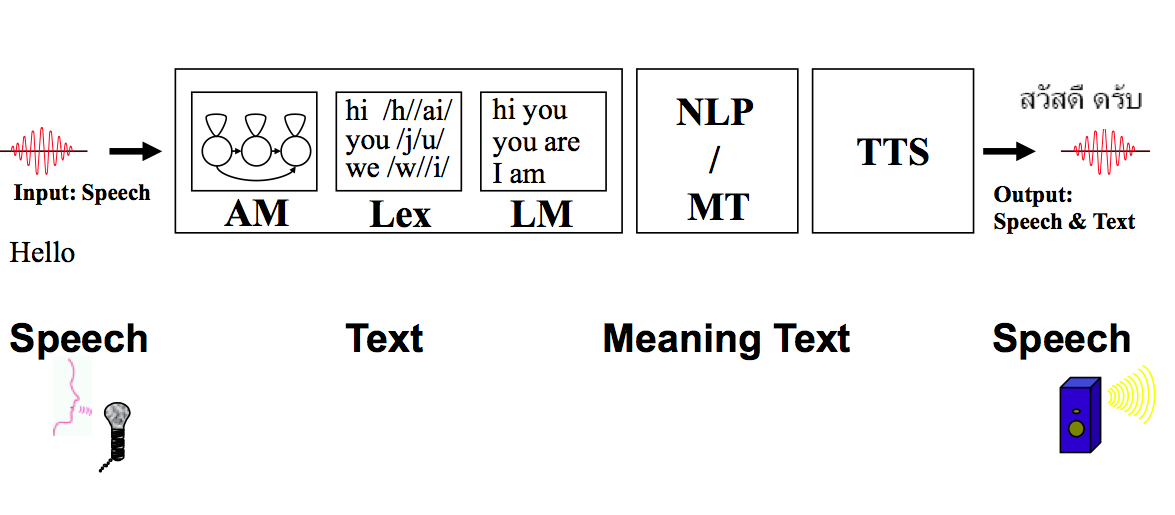
\includegraphics[width=10cm]{images/OverviewSchultz.png}
\caption{Overview according to Schultz}
\label{fig:overviewSchultz}
\end{figure}

\newpage

\section{Introduction}

\subsection{Why do we need Automatic Speech Recognition (ASR)?}

\begin{center}
  \begin{tabular}{ c | c }
    \hline
    Advantages & Disadvantages  \\ \hline
    Speech is a natural way of communication & When you are not allowed to speak, it is unusable   \\
    Allows an additional communication channel   & Unsatisfactory recognition rate  \\
    Hands and eyes are free for other tasks & Problems with accents, dialects and code-switching   \\
    Mobility & Cultural factors (e.g. uncertainty avoidance)   \\
    Some communication channels are speech-only & Speech input is still more expensive   \\
    \hline
  \end{tabular}
\end{center}

\begin{figure}[ht]
\centering
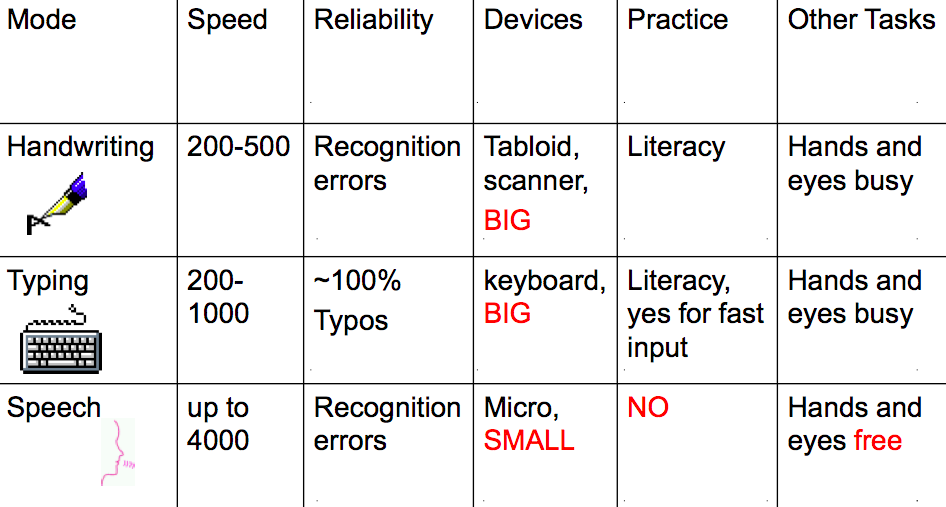
\includegraphics[width=10cm]{images/Input.png}
\caption{Input Characters per minute}
\label{fig:inputCharacters}
\end{figure}

\subsection{Where is Speech Recognition and Understanding useful?}
\subsubsection{Human-Machine Interaction}
\begin{enumerate}
\item Applications for Remote Control
\begin{itemize}
\item Using the phone to operate machines
\end{itemize}

\item Hands/eyes are busy or not usable
\begin{itemize}
\item Speech recognition while driving
\item Nurse bots for physically disabled
\end{itemize}

\item Authentication
\begin{itemize}
\item Speaker Identification/Verification/Segmentation
\item Language/Accent Identification
\end{itemize}

\item Entertainment

\item Indexing and Transcribing Acoustic Documents
\begin{itemize}
\item Archive, Summarize, Search and Data Retrieval
\end{itemize}

\end{enumerate}

\subsubsection{Human-Human Interaction}
\begin{enumerate}
\item Communication across language barriers
\begin{itemize}
\item Simultaniously translating one language into the other
\end{itemize}

\item Support human interaction
\begin{itemize}
\item Meeting and lecture systems
\item Speech therapy support

\end{itemize}


\end{enumerate}



\section{Basics}

\subsection{Speech units}

\begin{itemize}
    \item \textbf{phone}: a sound one produces, such as [p]
    \item \textbf{phoneme}: an abstract unit, such as /h/
    \item \textbf{morpheme}: the smallest part of speech with semantic meaning, for example un-break-able
\end{itemize}

When the meaning of an utterance can be changed by replacing one phone in the utterance with another phone, the replaced phone and the phone that replaces it are said to form a \textbf{minimal pair}.
A phoneme may correspond to one phone or a set of phones. In the latter case, all phones of the set are called \textbf{allophones} of the phoneme.
For example, /o/ and /u/ are phonemes in English because there are minimal pairs that differ only in these phonemes, such as ''bone`` and ''boon``. The English phoneme /p/ has two allophones, one with aspiration and one without it.

\subsection{$k$-means clustering}

Given an observation $(x_1, \ldots, x_n)$, find $k \leq n$ clusters $S = \left\{S_1, \ldots, S_k\right\}$, such that:

\[
    \argmin_S \sum\limits_{i = 1}^k \sum\limits_{x_j \in S_i} ||x_j - \mu_i||^2
\]

where $\mu_i$ is the mean of points in $S_i$.

\subsection{Comparing two utterances}

\begin{itemize}
    \item linear alignment
    \item dynamic time warping (DTW)
\end{itemize}

\section{Signal processing}

\subsection{Short-Term Spectral Analysis}

The general idea of short-term spectral analysis is to

\begin{itemize}
    \item multiply the speech signal with a window function
    \item apply the Discrete Time Fourier Transform (DTFT)
    \item use a filterbank (such as \textit{Mel} or \textit{Bark})
\end{itemize}

\subsection{Linear Predictive Coding}

LPC is an alternative to Fourier analysis. When using LPC, we assume that a speech signal is produced by a buzzer (\textit{glottis}) at the end of a tube (\textit{vocal tract}), with occasional added hissing and popping sounds. Then, the intensity and frequency can be estimated with linear prediction:

\begin{equation}
    \tilde{s}(n) = \sum\limits_{i = 1}^p \alpha_i s(n - i)
\end{equation}

Some sounds, for example nasal sounds, cannot be described by this model. This means that there will be an error, called the residue, which is stored and used to model other sounds:

\begin{equation}
    e(n) = s(n) - \tilde{s}(n)
\end{equation}

The goal of the prediction is to minimize the squared error $\sum e(n)^2$. This error can be further transformed into cepstral coefficients using the Z-transform.

\subsection{Cepstra}

The speech signal $s(n)$ can be described by a convolution of stimulating signal $u(n)$ (caused by the glottis) and an impulse response $h(n)$ (caused by the vocal tract and the lips):

\begin{equation}
    s(n) = u(n) \ast h(n)
\end{equation}

In speech analysis, we are particularly interested in discovering the formant structure. This means that we have to ''get rid`` of the stimulating signal:

\begin{equation}
    \mathcal{F}(s) = \mathcal{F}(u) \cdot \mathcal{F}(h)
\end{equation}

\begin{equation}
    \mathcal{F}^{-1}(\log(\mathcal{F}(s))) = \mathcal{F}^{-1}(\log(\mathcal{F}(u))) + \mathcal{F}^{-1}(\log(\mathcal{F}(h)))
\end{equation}

Note that after the inverse Fourier transform, we are not in the time domain, but in the cepstral domain. The lower cepstral coefficients describe the macro structure of the signal whereas the higher cepstral coefficients describe the micro structure of the signal. Thus, the higher cepstral coefficients are often discarded.

In order to separate the signal's components, we have to apply a \textit{lifter} to filter out the information we need. This is done by removing cepstral summits with a lowpass lifter.

\subsubsection{Mel-frequency cepstrum}

MFCCs are coefficients that collectively make up an MFC. MFCCs are commonly derived as follows:

\begin{enumerate}
    \item apply the Fourier transform to a signal
    \item apply a Mel filterbank
    \item take the $\log$ of the powers at each Mel ''bucket``
    \item take the discrete cosine transform (DCT) of the list of mel log powers
    \item the MFCCs are the amplitudes of the resulting spectrum
\end{enumerate}

Usually, we take the first coefficient (the power of the signal) and 12 more coefficients, amounting to a total of 13 numbers.

\subsection{Feature vectors}

During further processing, we often assume that the speech signal at a given point of time is independent from the signal before and after that point of time. This is a poor assumption. So, if we have a feature vector $x$ (if we're using MFCCs, we have 13 coefficients), we also store the first and second derivatives of $x$, namely $\Delta x$ and $\Delta \Delta x$ (if we're using MFCCs, we now have 39 numbers).

\section{Hidden Markov Models}

\subsection{The three great problems}

\subsubsection{Evaluation}

\textbf{Problem:} Given an HMM $\lambda$ and an observation $O = (x_1, \ldots, x_T)$, compute the probability $P(x_1, \ldots, x_T | \lambda)$.

\vspace{10pt}

\textbf{A weaker problem:} Given an HMM $\lambda$ an observation $O = (x_1, \ldots, x_T)$ and a state sequence $(s_{q_i}, \ldots, s_{q_T})$, compute the probability $P(x_1, \ldots, x_T | \lambda, (s_{q_1}, \ldots, s_{q_T}))$.

\vspace{5pt}

\textbf{Solution:}
\begin{equation}
    \pi(s_{q_1}) b_{q_1}(x_1) \prod\limits_{k = 1}^{T - 1} a_{q_{k}q_{k+1}} b_{q_{k+1}}(x_{k+1})
\end{equation}
This solution is of course not applicable to the evaluation problem because the state sequence is unknown.

\vspace{10pt}

\textbf{Solution: the Forward algorithm}. Define:

\begin{equation}
    \alpha_1(j) = \pi(s_j) \cdot b_j(x_1)
\end{equation}

\begin{equation}
    \alpha_t(j) = \sum\limits_i a_{ij} \cdot \alpha_{t-1}(i)
\end{equation}

\subsubsection{Decoding}

\textbf{Problem:} Given an HMM $\lambda$, and an observation $O = (x_1, \ldots, x_T)$, find the most likely state sequence $s_{q_1}, \ldots, s_{q_T}$:

\begin{eqnarray*}
    \argmax_{(q_1, \ldots, q_T)} P(q_1, \ldots, q_T \bigm| x_1, \ldots, x_T, \lambda)
    &=& \argmax_{(q_1, \ldots, q_T)} \frac{P(q_1, \ldots, q_T, x_1, \ldots, x_T \bigm| \lambda)}{P(x_1, \ldots, x_T \bigm| \lambda)} \\
    &=& \argmax_{(q_1, \ldots, q_T)} P(q_1, \ldots, q_T, x_1, \ldots, x_T \bigm| \lambda)
\end{eqnarray*}

\textbf{Solution: the Viterbi algorithm}. Define:

\begin{equation}
    z_1(j) = \pi(j) \cdot b_j(x_1)
\end{equation}

\begin{equation}
    z_t(j) = \max_i(a_{ij} \cdot z_{t-1}(i)) \cdot b_j(x_t)
\end{equation}

Both the Forward and the Viterbi algorithm often multiply many small numbers. This can lead to floating point underflow errors. As a solution, one can either scale the factor by a constant or use logarithms to turn the multiplications into additions.

\subsubsection{The Backward algorithm}

Obviously:

\begin{equation}
    P(x_1, \ldots, x_T \bigm| \lambda) = \sum\limits_i P(x_1, \ldots, x_T, q_t = i \bigm| \lambda)
\end{equation}

Define:

\begin{equation}
    \beta_t(i) = P(x_{t+1}, \ldots, x_T, q_t = i \bigm| \lambda)
\end{equation}

\vspace{10pt}

$\beta_t(i)$ is the probability of observing the partial observation $x_{t+1}, \ldots, x_T$ and being in state $s_i$. Then:

\begin{enumerate}
    \item Initialization: $\beta_T(i) = N^{-1}$
    \item Induction: $\beta_t(i) = \sum\limits_j a_{ij} \cdot b_j(x_{t+1}) \cdot \beta_{t+1}(j)$
    \item Termination: $P(x_1, \ldots, x_T \bigm| \lambda) = \sum\limits_j \beta_T(j)$ (shouldn't this be $\sum\limits_j \beta_1(j)$?)
\end{enumerate}

\subsubsection{Learning / optimization}

\textbf{Goal:} Given an observation $O$ and an HMM $\lambda$, find another HMM $\lambda'$ such that $P(O \bigm| \lambda') > P(O \bigm| \lambda)$.

\textbf{Solution:} We use the Baum-Welch algorithm, which is an EM algorithm (expectation-maximization). The Baum-Welch algorithm uses a forward-backward procedure.

First, define $\gamma_t(j)$, which is the probability that the system $\lambda$ is in state $s_j$ at time $t$ when producing the observation $X = (x_1, \ldots, x_T)$:

\begin{equation}
    \gamma_t(j) = \frac{P(q_t = j \bigm| X, \lambda)}{P(X \bigm| \lambda)} = \frac{\alpha_t(j) \cdot \beta_t(j)}{\sum\limits_i \alpha_t(i) \cdot \beta_t(i)}
\end{equation}

To optimize $a_{ij}$, we need the probability $\xi_t(i, j)$ of being in state $i$ at time $t$, transition from state $i$ to $j$ and be in state $j$ at time $t+1$.

\begin{eqnarray*}
    P(q_t = 1, q_{t+1} = j \bigm| X, \lambda) &=& \frac{P(q_t = 1, q_{t+1} = j, X \bigm| \lambda)}{P(X \bigm| \lambda)} \\
                                              &=& \frac{\alpha_t(i) \cdot a_{ij} \cdot b_j(x_{t+1}) \cdot \beta_{t+1}(j)}{P(X \bigm| \lambda)} \\
                                              &=& \xi_t(i, j)
\end{eqnarray*}

As a reminder (this follows from the rules of conditional probabilities):

\begin{equation}
    P(A \bigm| B, C) = \frac{P(A, B \bigm| C)}{P(B \bigm| C)}
\end{equation}

Define:
\begin{itemize}
    \item $\sum\limits_t \gamma_t(i)$ expected \# of times $i$ is visited
    \item $\sum\limits_t \xi_t(i, j)$ expected \# of transitions from $i$ to $j$
    \item $\pi(i)$ expected frequency in $i$ at time $(t = 1) = \gamma_1(i)$
    \item $a_{ij}$ expected \# transitions from $i$ to $j$ \textbf{div} expected \# of transitions from $i$
    \item $b_i(v_k)$ expected \# in $i$ and observing $k$ \textbf{div} expected \# in state $i$
\end{itemize}

Now, we can define the new HMM $\lambda' = (S, \pi', A', B', V)$:
\begin{itemize}
    \item $\pi'(i) = \gamma_1(i)$
    \item $a'_{ij} = \sum\limits_t \xi_t(i, j) \bigm/ \sum\limits_t \gamma_t(i)$
    \item $b'_i(v_k) = \sum\limits_t \gamma_t(i) \cdot \delta(x_t, v_k) \bigm/ \sum\limits_t \gamma_t(i)$ where $\delta(x, y) = (x \doteq y)$
\end{itemize}

Note that running the Viterbi algorithm leads to somewhat similar results. Training an HMM with Viterbi is faster, but when only little data is available, Baum-Welch performs better.

\subsection{HMM state tying}

When using Gaussian mixtures to model HMM output or transition probabilities, mixing more Gaussians doesn't necessarily lead to better results. This is due to an effect somewhat similar to overtraining.

\begin{itemize}
    \item we use a simple three-state bakis model (similar to left-right model) for each phone
    \item the $b_i(x)$ are often Gaussian mixtures
    \item discrete HMMs are rarely used
\end{itemize}

\subsubsection{Fully-continuous HMMs}
\begin{itemize}
    \item states that correspond to the same acoustic phenomenon share the same ''acoustic model``
    \item for example, all \textit{/g/} phonemes may share the same model for the \textit{g-b} HMM state
    \item the training data can be exploited better
    \item emission parameters can be estimated more robustly
    \item don't evaluate $b$ for every state - save computation time!
\end{itemize}
See also figure~\ref{fig:fullyContinuousHMMs}.
\begin{figure}[htb]
    \begin{minipage}{\linewidth}
        \vspace{6cm}
        \hfill \scriptsize hmm2.26
    \end{minipage}
    \caption{\label{fig:fullyContinuousHMMs} A fully-continuous HMM.}
\end{figure}

\subsubsection{Semi-continuous HMMs}
\begin{itemize}
    \item only one codebook of Gaussians in the system
    \item every acoustic model has its own set of \textit{mixture weights}
\end{itemize}
See also figure~\ref{fig:semiContinuousHMMs}.
\begin{figure}[htb]
    \begin{minipage}{\linewidth}
        \vspace{6cm}
        \hfill \scriptsize hmm2.27
    \end{minipage}
    \caption{\label{fig:semiContinuousHMMs} A fully-continuous HMM.}
\end{figure}

\subsubsection{Phonetically-tied semi-continuous HMMs}
One codebook per phone that is shared across polyphones. For example, \textit{/g/} might have one codebook and \textit{/ae/} another.

\subsection{HMM training}

A typical HMM training session might look like this:
\begin{enumerate}
    \item Initialization:
        \begin{itemize}
            \item initialize all parameters randomly
            \item or use pre-labeled data and compute initial parameters with e.g. \textbf{k-means}
        \end{itemize}
    \item Iterative optimization / training:
        \begin{itemize}
            \item for all training utterances, run \textit{Baum-Welch} and update the HMM accordingly
            \item continue for a defined number of iterations or until there are no more improvements
        \end{itemize}
    \item Evaluation by recording an utterance and testing the HMM.
\end{enumerate}

\subsection{HMM parameter initialization}

Use labeled data:
\begin{itemize}
    \item automatic labeling
        \begin{itemize}
            \item use an existing recognizer
            \item probably suboptimal
        \end{itemize}
    \item hand-made labels
        \begin{itemize}
            \item manually assign HMM states to speech frames
            \item probably time consuming
        \end{itemize}
    \item use partial labels
\end{itemize}

\section{Acoustic modeling}

\subsection{Discrete HMMs in continuous space}

In ASR terminology, an HMM is \textit{discrete} if the output space is partitioned into discrete, non-overlapping regions. The most common way to find such regions is to use $k$-means clustering. Then, the HMM states can emit discrete indices identifying one particular region.

A simple example of this is the regular partitioning of the F1-F2 formant space.

\subsection{Source coding}

\begin{itemize}
    \item Scalar quantization:
        \begin{itemize}
            \item for a scalar observation $x$, compute a quantization $y = Q(x)$
            \item can be simple, such as rounding (e.g. $1.3 \rightarrow 1.0$ or $1.3948 \rightarrow 1.40$)
        \end{itemize}
    \item Vector quantization:
        \begin{itemize}
            \item divide large set of vectors into groups using e.g. $k$-means clustering
            \item identify vectors by their group index
            \item lossy data compression
        \end{itemize}
\end{itemize}

\subsection{Continuous HMMs}

In ASR terminology, an HMM is \textit{continuous} when the output space is continuous and so are the emission probabilities $b_i$. Often, Gaussians $b_i = \mathcal{N}(\mu_i, \Sigma_i)$ are used ($\mu_i$ is a $k$-dimensional vector, $\Sigma_i$ is a $k \times k$ covariance matrix).

It is also possible to use a mixture of Gaussians:

\[
    b_i = \sum\limits_{j=1}^M c_{ij} \mathcal{N}(\mu_{ij}, \Sigma_{ij}) \mbox{\hspace{15pt} (or rather: \hspace{5pt}} b_i = \sum\limits_{j=1}^M c_{ij} \mathcal{N}(\mu_{j}, \Sigma_{j}) \mbox{\hspace{5pt} ?)}
\]

where $c_{ij}$ are the mixture weights.

If time is not an issue, we can use a continuous model. Otherwise, we will have to save computation time by altering our model.

\subsubsection{Conversion to semi-continuous model}

We ``pull out'' each Gaussian and collect them in a codebook. There will be a maximum of $M \cdot N$ Gaussians, where $N$ is the number of states.

\subsubsection{Conversion to shared semi-continuous model}

We extend the mixture weights to include Gaussians that were initially assigned to other states. This means that many mixture weights which previously were $0$ are now greater than $0$. This results in even more parameters.

\vspace{15pt}

\textbf{Problem:} If we create one codebook for each emission probability, we end up with \textit{a lot of} parameters. We may not have enough data to train our model.

\vspace{5pt}

\textbf{Solution:} Parameter tying. The most flexible way of parameter tying is to use an arbitrary number of Gaussian codebooks and an arbitrary number of mixture weight sets.

\subsubsection{Conversion to tied semi-continuous model}

Reduce the size of the codebook to a smaller size $L < M \cdot N$. Share Gaussians that belong to similar units (\textit{tie units}). This ``ties'' the codebook elements (and states) together. The number of models to train is now manageable.

\subsection{Parameter tying}

There are two main approaches to parameter tying:
\begin{itemize}
    \item \textbf{Knowledge driven:} Have an expert sit down and decide which parameters to tie.
    \item \textbf{Data driven:}
        \begin{itemize}
            \item let $n$ be the number of training vectors for a codebook, set the codebook size to $n \cdot f$ where $f$ is an empirically found factor
            \item run $k$-means with different values for $k$, choose the $k$ with the best result
            \item start with one codebook, train, once we have enough data, split
            \item start with huge codebook, remove Gaussians with too few training counts, retrain
            \item merge and split
        \end{itemize}
\end{itemize}

The following parameters can be tied:
\begin{itemize}
    \item sets of Gaussians
    \item within a mixture: have different Gaussians use the same covariance matrix
    \item transitions: different HMM states share the same transition probabilities
\end{itemize}

\subsection{Lexicon}

\textbf{Problem:} How do we connect our HMMs to words?

\vspace{5pt}

\textbf{Solution:} With a pronunciation dictionary.

\vspace{10pt}

In the simplest architecture, a word is represented as a sequence of phonemes and each HMM state represents one phoneme. In the lexicon, each word is bound to a phoneme sequence.

\subsubsection{Pronunciation variants}

One word can be pronounced differently due to:
\begin{itemize}
    \item coarticulation effects
    \item dialects (e.g. \textit{thing} vs. \textit{thang})
    \item various correct pronunciations (e.g. a = AE or a = EY)
    \item correct pronunciation differs from most commonly used ones (e.g. \textit{February} vs. \textit{Febyury})
\end{itemize}
To solve this problem, we add variants to the pronunciation dictionary. When building an HMM for a word, we build multiple, alternative state sequences.

\subsection{Context dependent acoustic modeling}

Consider the pronunciation of \textit{train} and \textit{tell}. Common lexicon entries will be \textit{T-R-EY-N} and \textit{T-EH-L}, but the actual pronunciation often sounds more like \textit{CH-R-EY-N} and \textit{T-HH-EH-L}. The phoneme \textit{T} sounds different depending on the phoneme following it.

At first, one might try to alter the lexicon entries, i.e. \textit{CH-R-UW} instead of \textit{T-R-UW}, but the \textit{CH} in \textit{true} sounds different from the one in \textit{church}.

So, we introduce new acoustic units, such that lexicon entries might look like \textit{T(R)-R-EY-N} and \textit{T(vowel)-EH-L}. This means that we use context-dependent models of the phoneme \textit{T}.

\subsubsection{Crossword context modeling}

It is not a good idea to assume that the left context of a word is silence. Because of this, we extend context modeling across word boundaries while building a sentence HMM.

\textit{Go to AM1 26/30 for more on this subject.}

\subsubsection{Position dependent modeling}

The same phoneme (with the same context) is pronounced differently depending on its position in the word. As an example, consider the \textit{D}-phoneme in \textit{Idaho} and \textit{my dad}. To solve this problem, we use position dependent modeling, where \textit{wb} indicates a word boundary. In \textit{Idaho}, this will become \textit{D(AY, AE)}, whereas in \textit{my dad}, it will become \textit{D(wb)(AY, AE)}.

\subsubsection{Parameter tying}

With so many different states, even with lots of training data, the HMM cannot be trained enough. As a solution, we use parameter tying to combine multiple contexts into the same context class:

\begin{itemize}
    \item Knowledge based:
        \begin{itemize}
            \item let a linguist define classes $C_i$ of phonemes (e.g. vowels, consonants, fricatives, etc.)
            \item then, define generalized triphones for a monophone $M$: $M(C_l, C_r)$
        \end{itemize}
    \item Data driven:
        \begin{itemize}
            \item use some algorithm with an optimization criterion to decide which contexts should be tied
        \end{itemize}
    \item Backoff procedure:
        \begin{itemize}
            \item if we have enough training data for triphones, use triphones $P_m(P_l, P_r)$
            \item otherwise, if we have enough training data for left or right context biphones ($P_m(P_l)$ or $P_m(P_r)$), use them
            \item otherwise, as a fallback, use an indepent model $P_m$
        \end{itemize}
\end{itemize}

\subsection{Clustering}

There are two different approaches to clustering:
\begin{itemize}
    \item \textbf{bottom-up clustering} (agglomerative): start with one class for each phone, then combine ``similar enough'' classes until satisified
    \item \textbf{top-down clustering} (divisive): start with one class for all phones, divide a class if it seems like a ``good idea'', continue until satisfied
\end{itemize}

Both approaches result in a \textit{clustering tree}.

\vspace{10pt}
\textbf{Problem:} How do we know whether it's a good idea to separate a class? 

\vspace{5pt}

\textbf{Solution:} Use a \textit{distance measure}.
\vspace{10pt}

\subsubsection{Continuous parametric models}
\begin{itemize}
    \item $d(f, g) = \int \min(f(x), g(x))$
    \item Kullback-Leibler divergence: $d_{KL}(f, g) = \int f(x) \ln \frac{f(x)}{g(x)}$
    \item entropy distance: $d(f, g) = H(f + g) - \frac{1}{2} H(f) - \frac{1}{2} H(g)$
\end{itemize}

\subsubsection{Discrete models}
Semi-continuous and discrete HMMs are represented by \textit{discrete} distributions.
\begin{itemize}
    \item $H(f) = \sum\limits_i f[i] \log_2(\frac{1}{f[i]})$
    \item $d(f, g) = H(f + g) - \frac{1}{2} H(f) - \frac{1}{2} H(g)$
    \item obviously: $f = g \Rightarrow H(f) = H(g) = H(f + g) \Rightarrow d(f, g) = 0$
\end{itemize}

As an example, consider $f = \left\{\frac{1}{2}, \frac{1}{2} \right\}$, $g = \left\{\frac{3}{4}, \frac{1}{4} \right\}$. Then, $f + g = \left\{\frac{5}{8}, \frac{3}{8} \right\}$. It follows that $H(f) = 1$, $H(g) \approx 0.81$, $H(f + g) \approx 0.95$ and finally $d(f, g) \approx 0.05$.

\vspace{10pt}

\textbf{Weighted discrete entropy distance}

\vspace{5pt}

Consider three models $M_1, M_f, M_{f^+}$, where $M_1$ is a model trained with many samples, $M_f$ is a model trained with few samples and $M_{f^+}$ is a model that is trained with few samples, but more than $M_f$ was trained with. Combining $M_1$ with $M_f$ should have a smaller impact on the distance compared to combining $M_1$ with $M_{f^+}$. Thus, we weigh the model entropy by the number of training samples:

\[
    d(f, g) = (n_f + n_g) H(f + g) - n_f H(f) - n_g H(g)
\]

\subsubsection{Kai-Fu Lee}
\begin{enumerate}
    \item train semicontinuous models for all three states of each triphone, e.g. triphone \textit{A(AE,K)-b} \textit{A(AE,K)-m} \textit{A(AE,K)-e}.
    \item initialize a context class for every triphone (a context class is defined by three distributions, e.g. \textit{$T_{17}$-b}, \textit{$T_{17}$-m}, \textit{$T_{17}$-e})
    \item compute all distances between different context classes of same phone:
        \[
            d(C_i, C_j) = E(C_i\mbox{\textit{-b}}, C_j\mbox{\textit{-b}}) + E(C_i\mbox{\textit{-m}}, C_j\mbox{\textit{-m}}) + E(C_i\mbox{\textit{-e}}, C_j\mbox{\textit{-e}})
        \]
    \item replace the two classes with the smallest class by their combination
    \item try to improve distance by moving any element from any class into any other class
\end{enumerate}

\vspace{10pt}
\textbf{Note:} This algorithm is completely data driven. Step 5 is expensive but important.
\vspace{10pt}

Kai-Fu Lee's algorithm produces \textit{generalized triphones}. For example, \textit{A(H,U)} and \textit{A(B,P)} might be combined into \textit{A37}, and \textit{A(L,N)} and \textit{A(M,M)} might be combined into \textit{A38}.

\subsubsection{Decision trees}

After clustering, we might end up with two classes:
\[
    C_1 = \left\{P_1(P_2, P_3), P_1(P_4, P_5) \right\} \mbox{\hspace{20pt}} C_2 = \left\{P_1(P_6, P_7), P_1(P_8, P_9) \right\}
\]
\textbf{Problem:} If we want to recognize the word sequence $P_3, P_1, P_7$, do we use $C_1$ or $C_2$ to model $P_1(P_3, P_7)$?

\vspace{5pt}

\textbf{Solution:} Build a decision tree.

\vspace{10pt}

\begin{enumerate}
    \item initialize one cluster containing all contexts
    \item for all clusters and questions: compute distance of subclusters
    \item perform the split that gets the largest separation
    \item continue until satisfied
\end{enumerate}

See figure~\ref{fig:growDecisionTree} for an example.

\begin{figure}[htb]
    \begin{minipage}{\linewidth}
        \vspace{5cm}
        \hfill \scriptsize am2.16
    \end{minipage}
    \caption{\label{fig:growDecisionTree} Growing the decision tree.}
\end{figure}

\textbf{Note:} It doesn't matter which questions we ask, as long as our question set allows for a variable enough separation.

\section{Language modeling}

Remember the fundamental problem of speech recognition:

\[
    \argmax_W P(X \bigm| W) \cdot P(W)
\]

The purpose of the language model is to compute the probability $P(W)$ of a word sequence $W = (w_1, \ldots, w_n)$. For example, the LM should compute that ''I owe you too`` is more likely than ''Eye O you two``.

The difficulty of recognizing a word sequence is correlated to the \textit{branching degree}. For example, the branching degree of \textit{``I apologize for being late, I'm very ---!''} is smaller than the one of \textit{``Hello, my name is ---.''}.

In formal language theory, $P(W)$ is either 0 or 1. This deterministic approach is unsuitable for ASR because spoken language has complex grammatical rules and is often ungrammatical, anyway.

Thus, we employ statistical methods. The choice of the next word depends on the entire history. Since there are too many histories to test them all, we have to find equivalence classes $\mathcal{C}$ so that:
\[
    P(w \bigm| \mbox{history}) = P(w \bigm| \mathcal{C}(\mbox{history}))
\]

A common choice for the equivalence classes are $n$-grams:
\[
    P'(w_k \bigm| w_1, \ldots, w_{k-1}) = P(w_k \bigm| w_{k - (n - 1)}, \ldots, w_{k-1})
\]

Usually, $P(w \bigm| \mbox{history})$ is estimated by counting relevant occurances:
\[
    P(w \bigm| \mbox{history}) = \frac{C(\mbox{history} \cdot w)}{C(\mbox{history})}
\]

A language model is ``good'' if it has a low \textit{perplexity}. The perplexity $PP$ of a language model $P$ on the test set $W = (w_1, \ldots, w_n)$ is:
\[
    PP = P(w_1, \ldots, w_n)^{-1/n}
\]

The key problem of $n$-grams is the \textit{data sparseness} problem: many n-grams will not occur in the training data, and many others will only occur very few times, resulting in inaccurate calculations. For example, in a several million word collection of English text, 50\% of trigrams occur only once, and 80\% of trigrams occur less than 5 times. As a start, we assign all strings a non-zero probability, in an effort to prevent ASR errors.

\subsection{Smoothing}

The idea of smoothing is to ``free probability mass'' from well-trained events and ``redistribute'' it to unseen events. This is somewhat similar to the idea of taxation.

\subsubsection{``Add-one'' smoothing}

Add 1 to all bigrams:

\begin{eqnarray*}
    P_{one}(w_i \bigm| w_{i - 1}) &=& \frac{C(w_{i-1}w_i)+1}{C(w_{i-1}) + n_v} \\
                                  &=& (1 - \lambda(w_{i-1})) \frac{C(w_{i-1}w_i)}{C(w_{i-1})} + \lambda(w_{i-1}) \frac{1}{n_v}
\end{eqnarray*}

where $\lambda(w_{i-1}) = n_v \bigm/ (n_v + C(w_{i-1}))$ and $n_v = \left|\left\{w : C(w) > 0 \right\} \cup \left\{\mbox{UNK} \right\}\right|$. This means that we're mixing the estimated distribution with the uniform distribution. However, when $n_v$ gets large, the estimation approximates the uniform distribution.

\subsubsection{Backoff smoothing}

Whenever possible, use higher-order models. Otherwise, for example with unseen events, backoff to lower-order models.
\begin{equation*}
    P_{bo}(w_i \bigm| w_{i-1}) = \begin{cases}
        \tilde{P}(w_i \bigm| w_{i-1}) & \mbox{if } C(w_{i-1}w_i) > 0 \\
        \lambda(w_{i-1}) \cdot P_{bo}(w_i) & \mbox{otherwise}
                                 \end{cases}
\end{equation*}

\vspace{20pt}
\textbf{Absolute discounting}
\vspace{10pt}

Subtract a fixed $D$ from each $n$-gram count:
\begin{equation*}
    P_{abs}(w_i \bigm| w_{i-1}) = \begin{cases}
        \frac{\max(C(w_{i-1}w_i)-D, 0)}{C(w_{i-1})} & \mbox{if } C(w_{i-1}w_i) > 0 \\
        \lambda(w_{i-1}) \cdot P_{abs}(w_i) & \mbox{otherwise}
                                 \end{cases}
\end{equation*}

\vspace{10pt}

\textit{\textbf{Note:} This formula is probably incorrect. I think what we're trying to do is something like this:
    \begin{equation*}
        P_{abs}(w_i \bigm| w_{i-1}) = \begin{cases}
            \frac{C(w_{i-1}w_i) - D}{C(w_{i-1})} & \mbox{if } C(w_{i-1}w_i) > D \\
            \lambda(w_{i-1}) \cdot P_{abs}(w_i) & \mbox{otherwise}
        \end{cases}
    \end{equation*}
    Or possibly even a weighted approach.
}

\vspace{20pt}
\textbf{Good-Turing estimation}
\vspace{10pt}

The idea is to reallocate the probability mass of $n$-grams that occur $r+1$ times in the training data to the $n$-grams that occur $r$ times. In particular, reallocate the probability mass of $n$-grams that were seen once to the $n$-grams that were never seen.

For each count $r$, we compute an adjusted count $r^\ast$:
\[
    r^\ast = (r+1)\frac{n_{r+1}}{n_r}
\]
where $n_r$ is the number of $n$-grams seen exactly $r$ times. Then, we compute the discount $d_r$:
\[
    d_r = \frac{r^\ast}{r}
\]

\vspace{20pt}
\textbf{Katz smoothing}
\vspace{10pt}

Use $k$ as a threshold to apply discounting. Use Good-Turing for discounting.
\begin{equation*}
    P_{katz}(w_i \bigm| w_{i-1}) = \begin{cases}
                                       \frac{C(w_{i-1}w_i)}{C(w_{i-1})} & \mbox{if } r > k \\
                                       d_r \cdot \frac{C(w_{i-1}w_i)}{C(w_{i-1})} & \mbox{if } k \geq r > 0 \\
                                       \alpha(w_{i-1}) \cdot P_{katz}(w_{i}) & \mbox{if } r = 0
                                   \end{cases}
\end{equation*}

\vspace{20pt}
\textbf{Kneser-Ney smoothing}
\vspace{10pt}

As an example, let's suppose that ``San Francisco'' is common, but ``Francisco'' occurs only after ``San''. Then ``Francisco'' will get a high unigram probability and so absolute discounting will give a high probability to ``Francisco'' appearing after novel bigram histories (for example, ``Los Francisco''). Since ``Francisco'' only ever occurs after ``San'', it is better to give it a low unigram probability. All in all, we use absolute discounting with a special backoff function. Define:
\begin{eqnarray*}
    \#(\bullet \; w_i) &=& \left|\left\{w_{i-1} : C(w_{i-1}w_i) > 0 \right\}\right| \\
    \#(\bullet \; \bullet) &=& \sum\limits_{w_i} \#(\bullet \; w_i)
\end{eqnarray*}

Then, define:
\[
    P_{KN}(w_i) = \frac{\#(\bullet \; w_i)}{\#(\bullet \; \bullet)}
\]

\subsubsection{Linear interpolation}

Define:
\[
    P_I(w_i \bigm| w_{i-2}w_{i-1}) = \lambda \cdot \tilde{P}(w+i \bigm| w_{i-2}w_{i-1}) + (1 - \lambda) \cdot P_I(w_{i} \bigm| w_{i-1})
\]

Key difference: in the case of non-zero counts, interpolated models still use information from lower-order models while backoff models do not.

\subsection{$n$-gram classes}

Another way to handle data sparsity is to group words into classes of similar semantic or grammatical behavior. For simplicity, let's assume that one word $w_i$ can be assigned to only one class $c_i$. Then:
\[
    P(w_i \bigm| c_{i-(n-1)}, \ldots, c_{i-1}) = P(w_i \bigm| c_i) \cdot P(c_i | c_{i-(n-1)}, \ldots, c_{i-1})
\]

$n$-gram classes have not improved recognition accuracy significantly.

\subsection{Different kinds of language models}

\subsubsection{Cache language models}
\begin{itemize}
    \item \textbf{Idea:} Use a static and a dynamic component.
    \item \textbf{Static component:} $P_S(w_k \bigm| w_{k-(n-1)}, \ldots, w_{k-1})$, i.e. the usual trained language model.
    \item \textbf{Dynamic component:} Complete $n$-gram language model constructed from the text dictated so far, e.g.:
        \[
            P_C(w_k \bigm| w_{k-(n-1)}, \ldots, w_{k-1}) = \frac{1}{2} \cdot f(w_k) + \frac{1}{4} \cdot f(w_k | w_{k-1}) + \frac{1}{4} \cdot f(w_k | w_{k-2} w_{k-1})
        \]
    \item \textbf{Total language model:} $P_T = \lambda_C \cdot P_C + (1 - \lambda_C) \cdot P_S$
    \item Compute $P_C$ on last $l$ words of cache, vary $\lambda_C$ with cache size.
\end{itemize}

\subsubsection{Trigger language models}
\begin{itemize}
    \item \textbf{Observation:} Often, when a content-carrying word occurs in a text, it is likely to occur again some time later.
    \item \textbf{Idea:} Use a standard interpolated $n$-gram model, but constantly update the unigram probabilities $P(w_k)$ for some words $w_k$.
    \item \textbf{Trigger:} For each word $w$ define a trigger list $L(w)$ of words that are likely to occur some time later, e.g. $L(\mbox{money}) = \left\{\mbox{bank}, \, \mbox{savings}, \, \mbox{dollars}, \, \ldots \right\}$
    \item Then, for each word $v \in L(w)$, increase $P(v)$ by some value.
\end{itemize}

\subsubsection{Multilevel language models}
\begin{itemize}
    \item \textbf{Idea:} Use language models $LM_W$ for word sequences, $LM_P$ for phrases and $LM_S$ for sentences trained as regular $n$-gram grammars over their corresponding segments of speech.
    \item \textbf{Combination:} Let the total language model $LM_T$ be a combination of the three models:
        \[
        LM_T = \lambda \cdot LM_W + \lambda \cdot LM_P + \lambda \cdot LM_S
        \]
\end{itemize}

\subsubsection{Interleaved language models}
Sentences can often be split into two separate word sequences, one containing \textit{content words} and the other containing \textit{non-content words}:
\[
\begin{array}{|r|ccccccc|}
    \hline
    \mbox{\textbf{sentence:}} & \mbox{The} & \mbox{president} & \mbox{of the} & \mbox{software company said} & \mbox{that they will} & \mbox{introduce} & \mbox{...} \\
    \hline
    \mbox{\textbf{non-content:}} & \mbox{The} & & \mbox{of the} & & \mbox{that they will} & & \mbox{...} \\
    \mbox{\textbf{content:}} & & \mbox{president} & & \mbox{software company said} & & \mbox{introduce} & \mbox{...} \\
    \hline
\end{array}
\]

Based on this, we define:
\[
    P(w \bigm| \mbox{history}) = \begin{cases}
        P_C(w \bigm| C_1(\mbox{history})) & \mbox{if $w$ is a content word} \\
        P_{NC}(w \bigm| C_2(\mbox{history})) & \mbox{if $w$ is a non-content word}
    \end{cases}
\]

\subsubsection{Morpheme-based language models}
In heavily inflicted or agglutinating languages, the word stem is succeeded or preceded by gender-, tempus-, numerus- and case-identifying elements. The probabilities of full words cannot be estimated robustly. However, a robust estimation can be given for the word stem. So, we don't compute the language model on sequences of words but on sequences of morphemes:
\[
    P(w_1, \ldots) = \tilde{P}(w_{11}, w_{12}, \ldots, w_{1n_1}, \ldots)
\]

\subsubsection{Context-free grammar language models}
Context-free grammars can be used instead of $n$-grams. The rules of the grammar can be written by an expert without the need for lots of training data. CFGs are powerful enough to represent large parts of natural languages and constrained enough to allow for efficient search space reduction. Furthermore, semantic analysis of speech is possible with CFG-derived finite state automata ($\to$ figure~\ref{fig:contextFreeGrammarLM}).

\begin{figure}[htb]
    \begin{minipage}{\linewidth}
        \vspace{4cm}
        \hfill \scriptsize lm2.9
    \end{minipage}
    \caption{\label{fig:contextFreeGrammarLM} Context-free grammar language models.}
\end{figure}

\subsubsection{Tree-based language models}
$n$-grams have a very limited context and training the parameters is almost impossible for large values of $n$. We can use a CART-based technique (classification and regression trees), where every tree node asks about $k$ previous words ($k \approx 20$). Every leaf node is a unigram probability distribution on our vocabulary. This is somewhat similar to clustering acoustic context-dependent models ($\to$ figure~\ref{fig:treeBasedLM}).

\begin{figure}[htb]
    \begin{minipage}{\linewidth}
        \vspace{4cm}
        \hfill \scriptsize lm2.10
    \end{minipage}
    \caption{\label{fig:treeBasedLM} Tree-based language models.}
\end{figure}

\subsubsection{HMMs for language modeling}

Often, speech is carried out in phases, such as \textit{greeting} $\rightarrow$ \textit{smalltalk} $\rightarrow$ \textit{good-bye}. Based on this, we can build an HMM, where every state emits language models or mixture weight distributions ($\to$ figure~\ref{fig:hmmLM}).

\begin{figure}[htb]
    \begin{minipage}{\linewidth}
        \vspace{3cm}
        \hfill \scriptsize lm2.11
    \end{minipage}
    \caption{\label{fig:hmmLM} HMMs for language modeling.}
\end{figure}

\subsection{Vocabulary selection}
A small vocabulary eliminates potentially confusing candidates and improves the word error rate. A larger vocabulary has a lower out-of-vocabulary rate, but the word error rate increases. The goal is to balance the WER and OOV rates. We do this by using a corpus of text to determine appropriate vocabularies. For example, we can pick data from a specific domain and use the most frequent words.

\subsection{$n$-gram pruning}
The size of higher-order $n$-gram models if often too large for practical applications. We can employ $n$-gram pruning to reduce the model size. Experience shows that trigram models can be pruned by more than 25\% without losing recognition accuracy.

\subsection{Problems with spontaneous speech}
\begin{itemize}
    \item silence between words (\textit{``hello world''} vs. \textit{``hello \hspace{5pt} world''})
    \item hesitations (\textit{``ah''}, \textit{``uhm''}, ...)
    \item filler words an phrases (\textit{``I mean''}, \textit{``you know''}, ...)
    \item false starts, aborts, etc. (\textit{``let's meet sun- no saturday''})
    \item non-verbal sounds (breathing, lip smacks, ...)
\end{itemize}

Possible solutions are:
\begin{itemize}
    \item just ignore it (\textit{duh!})
    \item increase context width (e.g. use $4$-grams instead of trigrams)
    \item skip spontaneous effects in the history
\end{itemize}

\subsection{Unknown words}

\vspace{5pt}
\textit{\textbf{Note:} Here, ``unknown word'' refers to a word not seen in the training data, but occuring in the decoder vocabulary and dictionary - as opposed to not being known at all.}
\vspace{10pt}

In the acoustic model, we can handle words that have not been seen in the training set by defining their pronunciation(s) in the pronunciation lexicon. However, in most speech recognition tasks, we cannot train all words that might have to be recognized some time. Approaches to this problem include:
\begin{itemize}
    \item rewrite all words in the training text that only occur one with UNK and treat every unknown word in the recognition run as UNK
    \item use a class-based language model and assign a class to every unknown word
    \item add new word into vocabulary and use cache language model to improve the parameters for subsequent recognitions
\end{itemize}

\subsection{OOV words}
OOV words are words that are not known at all. These words \textit{must} lead to recognition errors. Ideally, every OOV word causes only one substitution, which would imply WER = OOV. Usually, there are follow-up errors: every OOV word causes between 1.5 and 2 errors on average.

\subsection{Problems with different languages}
\begin{itemize}
    \item \textbf{Problem:} Highly inflecting languages pose more of a problem to language recognition. \textbf{Solution:} Use morpheme-based language models.
    \item \textbf{Problem:} Some languages, e.g. German allow arbitrary compounding of nouns. \textbf{Solution:} Decompose compound nouns.
    \item \textbf{Problem:} Some languages, e.g. Chinese have a different or no specified notion of words. \textbf{Solution:} Consider syllable-based language models.
\end{itemize}

\subsection{Language model adaptation}
Natural language is highly variable, depending on time (medieval German vs. current German), domain (fishing vs. politics), context (scientific paper vs. chatting with friends), etc.

\begin{figure}[htb]
    \begin{minipage}{\linewidth}
        \vspace{6cm}
        \hfill \scriptsize lm2.24
    \end{minipage}
    \caption{\label{fig:lmAdaptationFramework} Language model adaptation framework.}
\end{figure}

Generally, we have a large background corpus $\mathcal{B}$ and a small adaption corpus $\mathcal{A}$ depending on the current task. The goal is to compute a robust language model. We can try to solve this problem by using language model adaptation (see also figure~\ref{fig:lmAdaptationFramework}). There are three techniques of doing this:
\begin{itemize}
    \item model interpolation
    \item constraint specification
    \item meta-information extraction
\end{itemize}

\subsubsection{Retrieval of adaptation data}
We have to retrieve our adaption data froms somehwere:
\begin{itemize}
    \item Generate text using a grammar.
    \item Accumulate $\mathcal{A}$ during the recognition process.
    \item Use a small corpus $\mathcal{A}$ as a seed for retrieval techniques (online databases and WWW).
\end{itemize}

\subsubsection{Model interpolation}
\begin{enumerate}
    \item linear interpolation: $P(w_q \bigm| h_q) = (1 - \lambda) \cdot P_A(w_q \bigm| h_q) + \lambda \cdot P_B(w_q \bigm| h_q)$
    \item backoff:
        \[
            P(w_q \bigm| h_q) = \begin{cases}
                P_A(w_q \bigm| h_q) & \mbox{if } C(h_q w_q) \geq T \\
                \beta \cdot P_B(w_q \bigm| h_q) & \mbox{otherwise}
            \end{cases}
        \]
    \item dynamic cache model: $P(w_q \bigm| h_q) = \sum\limits_{\left\{c_q\right\}} P(w_q \bigm| c_q) \cdot P(c_q \bigm| h_q)$
    \item maximum a-posteriori:
        \[
            P(w_q \bigm| h_q) = \frac{\epsilon \cdot C_A(h_qw_q) + C_B(h_qw_q)}{\epsilon \cdot C_A(h_q) + C_B(h_q)}
        \]
\end{enumerate}

\subsubsection{Constraint specification}
\textbf{Idea:} Extract features from corpus $\mathcal{A}$ that are used as constraints for the adapted SLM.
\subsubsection{Meta-information extraction}
\textbf{Idea:} Use corpus $\mathcal{A}$ to extract background information about the underlying subject matter. Improve upon the background model based on semantic classification.

\section{Search}

\textbf{Isolated word recognition:}
\begin{itemize}
    \item for every applicable vocabulary word, compute it's score (DTW) and it's likelihood (Forward algorithm)
    \item report the word with the best score / likelihood
\end{itemize}

\vspace{5pt}

\textbf{Continuous speech recognition:}
\begin{itemize}
    \item not only find state sequence in words
    \item but also find the word sequence
\end{itemize}

\vspace{5pt}

\subsection{DTW optimization}
\begin{itemize}
    \item define start and end point
    \item path should be close to diagonal
    \item no two successive horizontal / vertical steps
    \item pruning: eliminate losers (with score $s < s_{best} - \Delta$)
    \item usually, we're only interested in the final score, so we can overwrite older values
\end{itemize}

Drawbacks of DTW include speaker dependency and inefficiency for large vocabularies.

\subsection{Viterbi optimization}
Use tree search ($\to$ figure~\ref{fig:viterbiTreeSearchOptimization}).
\begin{figure}[htb]
    \begin{minipage}{\linewidth}
        \vspace{5cm}
        \hfill \scriptsize search1.17
    \end{minipage}
    \caption{\label{fig:viterbiTreeSearchOptimization} Viterbi tree search optimization.}
\end{figure}

\subsection{Advanced optimization techniques}

\subsubsection{Two-level DTW}
\begin{enumerate}
    \item for each remotely likely word begin time, compute DTW with open end within all words
    \item for each word start and end times calculated in the previous step, combine words with DTW based on calculated scores
\end{enumerate}

Obviously, this is extremely costly for large vocabularies and longer words.

\subsubsection{Depth-first search}

Depth-first vs. breadth-first corresponds roughly to \textit{time-asynchronous} vs. \textit{time-synchronous}.

\textbf{$A^{\ast}$ search} (usually implemented with a stack decoder):

\subsubsection{Viterbi beam search vs. $A^{\ast}$ stack decoder}
Beam search doesn't require a heuristic and it is appropriate for parallel implementation. However, it is not admissible, that is it might not find the best solution. Nowadays, beam search is usually preferred over $A^{\ast}$ (though $A^{\ast}$ is taken for search through $n$-best and lattice structures).

\subsubsection{One stage dynamic programming}
Use Viterbi within words. For the first state of each word, consider the best last state of all words as predecessor. In order to reconstruct the best word sequence, find the best predecessor word to the current word. Finally backtrace.

\textit{\textbf{Note:} ???}

All search techniques use two strategies for efficiency:
\begin{itemize}
    \item \textbf{Sharing:} Keep intermediate results so that they can be reused by other paths without recomputation. For example, when computing the emission probabilities of \textit{``can''} and \textit{``cash''}, we can reuse the emission probabilities for the phonemes \textit{C} and \textit{AE}.
    \item \textbf{Pruning:} Disregard unpromising paths without wasting time exploring them further.
\end{itemize}

When using bigrams, the best predecessor depends only on the current word, this is possible by storing one backpointer for each active word end. When using trigrams, the best predecessor also depends on the successor of the current word. Then, things ``get ugly'' and we have to approximate a solution.

The transition into an initial state of a word $Z$ is computed by maximizing (Viterbi / DTW) the scores / accumulated distances $C(W)$ of all word-final states in the previous time frame and adding the local acoustic score $am(Z)$: e.g. $C(X) + am(Z)$ vs. $C(Y) + am(Z)$. When using a grammar, we additionally have to add to the accumulated score a language model score $lm(Z)$, e.g. $C(X) + am(Z) + lm(X, Z)$ vs. $C(Y) + am(Z) + lm(Y,Z)$. Without a grammar, the best predecessor state is the same for all word-initial states, whereas with a grammar, the best predecessor state also depends on the word transition probability.

\vspace{10pt}

When using tree search with a language model, we have a problem. After making a word-to-word transition, we don't know which word we are entering, but this knowledge is required to properly compute the probability of the transition. The solution to this are \textbf{delayed bigrams}. We make every word's final state unique. That way, we know which word we processed when we are in the final state. At that point, we can incorporate the language model information into our calculation (hence,
\textit{delayed}) ($\to$ figure~\ref{fig:delayedBigrams}).
\begin{figure}[htb]
    \begin{minipage}{\linewidth}
        \vspace{4cm}
        \hfill \scriptsize search2.15
    \end{minipage}
    \caption{\label{fig:delayedBigrams} Delayed bigrams.}
\end{figure}

\vspace{10pt}

\subsubsection{Unigram lookahead}
No bigram information can be included until word identity is known. Instead, we estimate the unigram information of the remainder subtree and include the bigram information as soon as possible (see also figure~\ref{fig:unigramLookahead}).
\begin{figure}[htb]
    \begin{minipage}{\linewidth}
        \vspace{4cm}
        \hfill \scriptsize search2.16
    \end{minipage}
    \caption{\label{fig:unigramLookahead} Unigram lookahead.}
\end{figure}

\vspace{10pt}

\subsubsection{Multi-pass searches}
Why use multiple passes in continuous speech recognition:
\begin{itemize}
    \item we could use a good estimator for $A^{\ast}$ search
    \item in pruning we could use a good lookahead to prune away the ``right'' parts
    \item recover from errors resulting from delayed bigrams
\end{itemize}
Forward-backward search: first, run backward pass, then run forward pass using backward scores to do pruning. Problems:
\begin{itemize}
    \item when using a search pass to compute information for pruning, it has to be a lot faster than the actual search pass
    \item it cannot produce better results than the actual search pass
    \item no runon recognition possible (start processing before sentence has finished)
    \item where do we get backward bigrams from?
\end{itemize}
Example for a multi-pass search: in the first pass, use a narrow beam and a fast but weak acoustic model to prune some paths. In the second pass, use a regular Viterbi search with a wider beam and a slower but more powerful acoustic model, considering that some areas have already been pruned in the first run.

\subsubsection{Multiple hypothesises}
Reasons:
\begin{itemize}
    \item do postprocessing on all hypothesises using additional knowledge
    \item speech understanding
    \item manual recovery options for the users
\end{itemize}
When recognizing isolated words, simply report not only the best, but the $n$ best results. In continuous speech recognition, we can either use multiple recognizers and report all their results, or let Viterbi not only remember the best predecessor, but the $n$ best predecessors.

A problem with multiple hypothesises is that the results are often quite similar in respect to their content words, while the non-content words are more variable. This results in many ``useless'' hypothesis. But if we simply increase $n$, the system may become too slow. The solution to this is to use \textbf{word lattices} ($\to$ figure~\ref{fig:wordLattice}).
\begin{figure}[htb]
    \begin{minipage}{\linewidth}
        \vspace{3cm}
        \hfill \scriptsize search2.22
    \end{minipage}
    \caption{\label{fig:wordLattice} A word lattice.}
\end{figure}

\section{Text-to-speech synthesis}

Typically, text-to-speech synthesis involves three steps:
\begin{enumerate}
    \item \textbf{text analysis:} from strings of characters to words
    \item \textbf{linguistic analysis:} from words to pronunciations and prosody
    \item \textbf{waveform synthesis:} from pronunciations to waveforms
\end{enumerate}

We use the \textit{mean mel cepstral distortion} (\textbf{MCD}) as a quality measure (smaller is better).

\subsection{Text analysis}
\begin{itemize}
    \item character encodings
    \item word segmentation
    \item numbers, symbols, non-standard words
        \begin{itemize}
            \item anything not directly in the lexicon
            \item OOV or novel forms
            \item abbreviations, letter sequences, acronyms
        \end{itemize}
    \item may require special rules
        \begin{itemize}
            \item train rules for homographs
            \item numbers, roman numerals
        \end{itemize}
\end{itemize}
Text processing errors are the most common complaints in TTS. Examples:
\begin{itemize}
    \item ``My cat who \textit{lives} dangerously has nine \textit{lives}.''
    \item ``He stole \textit{\$}100 from the bank.''
    \item ``He stole \textit{1996} cattle on 25 Nov. \textit{1996}.''
    \item ``It's 13 \textit{St.} Andrew \textit{St.} near the bank.''
\end{itemize}
We employ a ``bunch of hacky rules'':
\begin{itemize}
    \item \textbf{splitter:} domain-independent tokenizer
    \item \textbf{token type classifier:} identify numbers and abbreviations, disambiguate homographs
    \item \textbf{token type expander}
    \item \textbf{language model}
\end{itemize}

\subsection{Linguistic analysis}

The lexicon should be as comprehensive as possible, but this is impossible. So, we have to pronounce OOV words, too.

\subsubsection{Bootstrapping}

\begin{enumerate}
    \item select some frequently occuring words and build lexical entries from them
    \item select an article of text
    \item synthesize each unknown word, add correct words to list
    \item repeat
\end{enumerate}

\subsection{Waveform synthesis}
Concatinative synthesis:
\begin{itemize}
    \item random word / phrase concat
    \item phone concat
    \item diphone concat ($\left|\mbox{phones}\right|^2$ transitions)
    \item sub-word unit selection
    \item cluster-based unit selection
\end{itemize}

\section{Spoken dialog systems}

A dialog is a verbal interaction of two or more agents over more than one utterance in order to establish a joint goal. A spoken dialog system is an autonomous, artificial system that engages in a dialog with a human and employs speech recognition and synthesis. Commonly, a complete interaction is referred to as a \textit{session}, an \textit{utterance} is one person's speech between two pauses, and a \textit{turn} represents all utterances of one partner, until the other partner starts interacting. A \textit{barge-in} happens when a turn is interrupted.
There are two kinds of initiatives, the \textit{system initiative}, e.g. ``Please tell me your destination airport.'' (more rigid, less ASR errors) or the \textit{mixed initiative}, e.g. ``What flight are you interested in?'' (less rigid, harder to recognize and understand).

\begin{figure}[htb]
    \begin{minipage}{\linewidth}
        \vspace{5cm}
        \hfill \scriptsize sds.7
    \end{minipage}
    \caption{\label{figureA} Components of a spoken dialog system.}
\end{figure}

A \textit{discourse} is the entirety of information and structure of the ongoing dialog up to a certain point. Each new utterance must be interpreted in the light of the ongoing discourse and then included in it.

\vspace{5pt}

In order to represent a discourse, Montague grammars are commonly used (transform text into first order logic). Problem: ``A man walks in the park. He whistles'' $\rightarrow (\exists x : man(x) \wedge walksinpark(x)) \wedge (\exists x : whistles(x))$. What we need is \textit{anaphora resolution}.

\vspace{5pt}

Don't forget \textit{typed feature structures}. We can build \textit{semantic grammars} with it.

\vspace{5pt}

\textbf{Dialog strategies:}
\begin{itemize}
    \item \textbf{plan-based} system: the idea is that communication is the result of a plan (to do / achieve something)
    \item \textbf{grammar-based} system: there are adjacency pairs, such as \textit{question} $\rightarrow$ \textit{answer}, \textit{proposal} $\rightarrow$ \textit{acceptance}, etc.
    \item \textbf{finite-state grammars:} describe possible events with a finite state automata (simple to produce, but rigid)
    \item \textbf{rational agency:} formally describe rational behavior and then use formal proofs in order to deduce next steps
    \item \textbf{frame-based} systems: somewhat similar to web forms, additionally define \textit{moves} (which may contain \textit{conditions}) to ask for specific information
    \item \textbf{statistical systems:} learn optimal next system action from corpus of completed dialogs
\end{itemize}

\vspace{5pt}

The dialog system has to communicate with the ASR system. Returning only the best hypothesis is usually not sufficient. We may have to weigh hypothesises according to the dialog act expectations. Also, we should adapt the context to each turn (e.g. in a navigation system in Karlsruhe, \textit{``Durlach``} will be more likely than \textit{``Paris''}, which is different from most other contexts).

\vspace{5pt}

If our system is \textit{multimodal}, we can also use gestures, etc.

\section{Multilingual speech processing}

We can't simply retrain on foreign data, because:
\begin{itemize}
    \item different scripts, no vowelization, no writing system
    \item no word segmentation, rich morphology
    \item tonality, click sounds
    \item social factors such as trust, access, exposure and cultural background
\end{itemize}
For an overview of the system, see figure~\ref{fig:overviewMSPS}.

\begin{figure}[htb]
    \begin{minipage}{\linewidth}
        \vspace{7cm}
        \hfill \scriptsize msp2.4
    \end{minipage}
    \caption{\label{fig:overviewMSPS} Overview of multilingual speech processing systems.}
\end{figure}

Let's try to build a language independent ASR system!
\begin{itemize}
    \item language independent acoustic modeling
        \begin{itemize}
            \item \textit{International Phonetic Alphabet} easy to implement, easy to port to other languages
            \item fully data-driven procedure
        \end{itemize}
    \item universal language model: combine LMs of different languages to allow code switching
\end{itemize}

\vspace{10pt}
\textbf{Multilingual acoustic modeling}
\vspace{10pt}

\begin{enumerate}
    \item \begin{itemize}
            \item uniform multilingual speech database
            \item monolingual recognizers for many languages
        \end{itemize}
    \item \begin{itemize}
            \item combine monolingual acoustic models
            \item share data across languages
        \end{itemize}
\end{enumerate}

\vspace{10pt}
\textbf{Acoustic model combination}
\vspace{10pt}

Sound production is \textit{human}-specific, not \textit{language}-specific. Thus, it is sufficient to represent sounds with the IPA.
\begin{enumerate}
    \item build universal sound inventory based on IPA (485 sounds $\rightarrow$ 162 IPA sound-classes)
    \item each sound class is represented by one phoneme which is trained through data sharing:
        \begin{itemize}
            \item \textit{m}, \textit{n}, \textit{s}, \textit{l} occur in all languages
            \item \textit{a}, \textit{e}, \textit{i}, \textit{o}, \textit{u} and \textit{p}, \textit{b}, \textit{t}, \textit{d}, \textit{k}, \textit{g}, \textit{f} occur in most languages
            \item some data is not shared
        \end{itemize}
\end{enumerate}

\vspace{10pt}
\textbf{Challenges}
\vspace{5pt}

\begin{itemize}
    \item Many ASR algorithms are language independent, but they require lots of training data. For many languages, not a lot of training data exists, so we need a different approach. For example, we might use intelligent learning systems.
    \item The contexts of sounds are language specific. How can we still use context dependent modeling?
        \begin{itemize}
            \item multilingual decision context trees
            \item specialize decision tree by adaptation
        \end{itemize}
\end{itemize}

\vspace{10pt}
\textbf{Web-derived pronunciations}
\vspace{5pt}

\vspace{10pt}
\textbf{Unsupervised training}
\vspace{5pt}

Idea: decode untranscribed audio data, select data with high confidence, use selected data to train / adapt recognizer.

\newpage
\section{Prüfungsfragen}
\subsection{Allgemeine Fragen}
\begin{itemize}
\item Was ist MMMK? Wofür steht MMMK?
\begin{itemize}
\item \emph{Multilinguale Mensch-Maschine Kommunikation}
\end{itemize}
\item Wo findet MMMK Anwendung?
\begin{itemize}
\item \emph{Interaktion mit einem Computer/Maschine  mittels natürlicher Sprache}
\end{itemize}
\item Vor- und Nachteile gegenüber anderen Kommunikationsmitteln
\begin{itemize}
\item \emph{siehe Vor- und Nachteile im Kapitel 1} %variabel machen
\end{itemize}
\item Welche Probleme können dabei auftreten?
\item Zeichnen sie das Blockschaubild (Young oder Schultz)
\begin{itemize}
\item \emph{siehe Overview Figure 1 und 2} % variabel referenzieren 
\end{itemize}
\item Geben Sie die Fundamentalformel (nach Bayes) an.
\begin{itemize}
\item $\hat{W} = argmax_{W} P(W | X) = argmax_{W} \frac{P(X|W) \cdot P(W)}{P(X)}$ 
\end{itemize}
\item Beschreiben Sie den Zusammenhang zwischen Fundamentalformel und Blockschaltbild.
\begin{itemize}
\item\emph{$P(X|W)$ kommt vom Akustischen Modell, $P(W)$ vom Sprachmodell, $P(X)$ ist die a-priori Wahrscheinlichkeit, 
$argmax$ ist der Decoder und $\hat{W}$ die wahrscheinlichste Hypothese.}
\end{itemize}
\item Was ist an Umgangssprache so schlimm?
\begin{itemize}
\item \emph{Grammatisch oft inkorrekt, Aussprache ggf. undeutlich bzw. untypisch}
\end{itemize}
\end{itemize}

\subsection{Vorverarbeitung}
\begin{itemize}
\item Erklären sie die Funktionsweise eines Kondensatormikrophons.
\begin{itemize}
\item \emph{Zwei Membranen, eine dicke und eine dünne, die als Plattenkondensator fungieren. Die dünne Membran wird durch Schalldruckwellen angeregt und schwingt. Durch die Kapazitätsänderung kommt es zu einer messbaren Spannungsänderung.}
\end{itemize}
\item Was macht man bei der Vorverarbeitung?
\begin{itemize}
\item \emph{Quantisierung, Abtasten (Sampling) [Diskret] $\rightarrow$ Fouriertransformation um an Frequenz- und Zeitinformation zu gelangen.} 
\end{itemize}
\item Was muss beim Abtasten (Sampling) beachten?
\begin{itemize}
\item \emph{Nyqist-Theorem: Abtastfrequenz muss echt größer als der doppelten Signalfrequenz sein.}
\end{itemize}
\item Was machen Quantisierung und Sampling?
\begin{itemize}
\item \emph{Quantisierung diskretisiert die Y-Achse und Sampling die X-Achse.}
\end{itemize}
\item Was für ein Filter wird beim Sampling benötigt und warum?
\begin{itemize}
\item \emph{Tiefpassfilter, da wir ein bandbegrenztes Signal brauchen.}
\end{itemize}
\item In welchem Frequenzbereich hört der Mensch?
\begin{itemize}
\item \emph{bis zu 32k Hz, Abtastfrequenz ist üblicherweise 8kHz}
\end{itemize}
\item Warum wollen wir die Frequenzinformation haben?
\begin{itemize}
\item \emph{Das Ohr macht das auch so.}
\end{itemize}
\item Was macht man nach dem Digitalisieren des Signals?
\begin{itemize}
\item \emph{Nach der Digitalisierung wird das Signal gefenstert.}
\end{itemize}
\item Was wird beim Fenstern gemacht? Und warum wird das Signal gefenstert?
\begin{itemize}
\item \emph{Hier muss noch die Antwort rein. TADASDASDA}
\end{itemize}
\end{itemize}


\subsection{Akkustisches Modell}


\subsection{Sprachmodell}


\newpage

\begin{figure}
\centering
\textbf{Danksagung} \\
\textbf{Guido Brückner} für die Kapitel Overview, Basics, Signal processing, Hidden Markov Models, Acoustic modeling, Language modeling, Search, Text-to-speech synthesis, Spoken dialog systems und Multilingual speech processing
\end{figure}

\end{document}
